% Source - https://tex.stackexchange.com/a/722311
% Posted by Qrrbrbirlbel
% Retrieved 2026-04-03, License - CC BY-SA 4.0

\documentclass[tikz]{standalone}
\usetikzlibrary{nfold}
\makeatletter
\tikzset{offset/.code=\tikz@addmode{\pgfgetpath\tikz@temp\pgfsetpath\pgfutil@empty\pgfoffsetpath\tikz@temp{#1}}}
\makeatother
\tikzset{
  double circle/.style 2 args={
    shape=circle,postaction={draw,#2,offset={#1}}},
  double circle/.default={2pt}{blue},
  double circle*/.style 2 args={
    double circle={#1}{#2},
    /pgf/outer xsep/.expanded={\pgfkeysvalueof{/pgf/outer xsep}+max(0,-(#1))},
    /pgf/outer ysep/.expanded={\pgfkeysvalueof{/pgf/outer ysep}+max(0,-(#1))}},
  double circle*/.default={2pt}{blue}}
\begin{document}
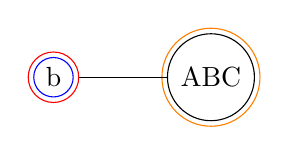
\begin{tikzpicture}
\node (A) [double circle, draw=red] {b};
\node (B) at (2,0) [draw, double circle={-2pt}{orange}] {ABC};
\draw (A) -- (B);
\end{tikzpicture}

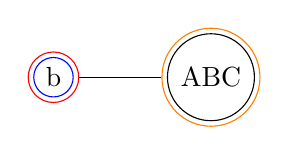
\begin{tikzpicture}
\node (A) [double circle, draw=red] {b};
\node (B) at (2,0) [draw, double circle*={-2pt}{orange}] {ABC};
\draw (A) -- (B);
\end{tikzpicture}
\end{document}
